%!TEX root = ../../../memoria.tex
\section{Carro Compra}
	El carro de compra agrupa todos los productos seleccionados para efectuar la compra. Actualmente del carro de compra se pueden desprender dos acciones: \nameref{chapter:section:carro_compra:subsection:add} y \nameref{chapter:section:carro_compra:subsection:request}.

	\subsection{Agregar elementos al carro}\label{chapter:section:carro_compra:subsection:add}
		El proceso de agregar elementos es muy sencillo, simplemente hay que ir a la vista de un producto, ir donde esta el botón \addtocartLABEL, seleccionar la cantidad de productos que se desean agregar y finalmente apretar el botón. En la \refFigura{figure:solution:cart:button} se han seleccionado 4 productos para agregar al carro.

		\begin{figure}[H]
			\centering
			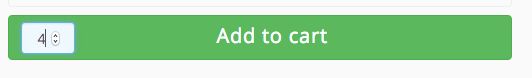
\includegraphics[width=0.8\textwidth]{figuras/solution/cart/button.png}
			\caption{Botón para agregar productos al carro. En la figura se han seleccionado 4 productos iguales para agregar al carro de compra.}
			\label{figure:solution:cart:button}
		\end{figure}

		Una vez agregado al carro, el número de elementos presentes en el carro de compra se actualiza. Este número es visible en la parte superior izquierda de la interfaz (\refFigura{figure:solution:cart:header}).

		\begin{figure}[H]
			\centering
			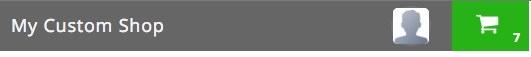
\includegraphics[width=0.8\textwidth]{figuras/solution/cart/header.png}
			\caption{Icono que muestra la cantidad de elementos que tiene el carro. El icono del carro es un bottón para la vista del carro.}
			\label{figure:solution:cart:header}
		\end{figure}

		El estado del carro de compra se guarda en la base de datos, esto quiere decir que aunque haga \logoutCPT, el estado seguira vigente para la próxima vez que haga \loginUpperCPT.


	\subsection{Consultar los elementos del carro}\label{chapter:section:carro_compra:subsection:request}
		El icono del carro de compras que se aprecia en la \refFigura{figure:solution:cart:header} es a su vez un botton, el cual muestra todos los elementos agregados al carro en una lista horizontal (\refFigura{figure:solution:cart:view}). Además muestra un resumen de la compra con la siguiente información:
		\begin{itemize}
			\item
				Cantidad de elementos.
			\item
				Sub total.
			\item
				Costos de envio.
			\item
				Impuestos
			\item
				Total
		\end{itemize}


		\begin{figure}[H]
			\centering
			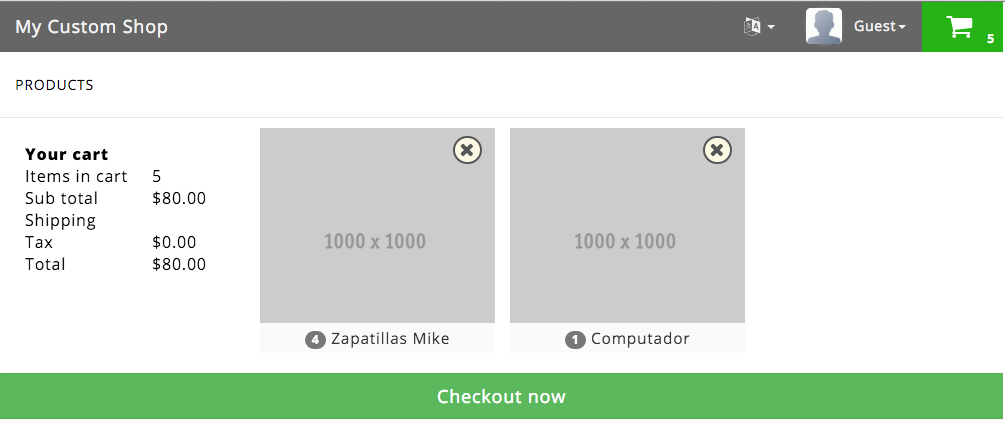
\includegraphics[width=0.8\textwidth]{figuras/solution/cart/view.png}
			\caption{Información global del carro. Tiene un resumen del costo total de los elementos seleccionados.}
			\label{figure:solution:cart:view}
		\end{figure}

		Es posible sacar productos del carro simplemente presionando sobre la [x] que se observa en la esquina superior derecha de cada producto (\refFigura{figure:solution:cart:product}). Así es posible retractarse de la compra de algunos productos.

		\begin{figure}[H]
			\centering
			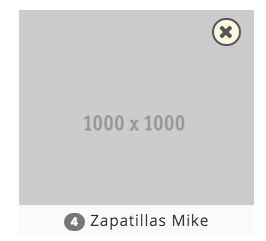
\includegraphics[width=0.5\textwidth]{figuras/solution/cart/producto.png}
			\caption{Vista básica de un producto seleccionado. La [x] de la esquina superior derecha permite eliminar ese producto del carro de compra.}
			\label{figure:solution:cart:product}
		\end{figure}

		El botón \checkoutNowLABEL que se ubica en la parte inferior de la vista \nameref{chapter:section:carro_compra:subsection:request} nos envía a la vista de \nameref{chapter:solucionimplementada:section:shipping}.

		No es posible elegir la cantidad de elementos de un determinado producto para eliminar. En el caso del producto de la \refFigura{figure:solution:cart:product}, solo se pueden eliminar los 4 productos simultaneamente.


